\documentclass{report} \input{preamble} \input{macros} \input{letterfonts}
\title{\Huge{AP Physics}\\Electricity and Magnetism}
\author{\huge{Ben Feuer}}
\date{2023}

\begin{document}

\maketitle

\newpage% or \cleardoublepage
% \pdfbookmark[<level>]{<title>}{<dest>}
\pdfbookmark[section]{\contentsname}{toc}
\tableofcontents


%
\chapter{Electric Fields and Forces}
%

\nt{This is a compilation of notes for Electricity and Magnetism for my AP Physics class. 
  \\
  Much of the content is taken from the textbook \textit{College Physics: A Strategic Approach} by Knight, Jones, and Field, specifically  chapters 20 to 24 or from my physics class that is taught by Thomas J. Erickson \url{mailto:terickson@mxschool.edu}
}

\section{Equations for Electric Fields and Forces}

\begin{itemize}
  \item $ m_{electron} = 9.11* 10^{-31} $ 
  \item $ m_{proton} = 1.67* 10^{-27}$
  \item $ q_{electron} = -1.6 * 10^{-19} C $ 
  \item $ q_{proton} = +1.6 * 10^{-19} C $
  \item $ F_{1 on 2} = F_{2 on 1} = \frac{k*q_1*q_2}{r^2} $
  \item $ E = \frac{F_{on q}}{q} $ 
  \item $ E = \frac{kQ}{r^2} $ 
  \item $ E_{capacitor} = \frac{Q}{\epsilon_0A} $
  \item $ k = 9.0 * 10^9 \frac{N \cdot m^2}{C^2} $
  \item $ \epsilon_0 = 8.85 * 10^{-12} \frac{C^2}{N\cdot m^2} $
\end{itemize}


\section{Charges and Forces}

\begin{itemize}
  \item Frictional forces, such as rubbing, add something called charge to an object or remove it from the object. The process itself is called charging. More vigorous rubbing produces a larger quantity of charge.
  \item There are two kinds of charges: positive and negative
  \item Two objects with the same charge repel each other while two objects with differing charges attract each other. The forces of repulsion and attraction here are called \textit{electric forces}. 
  \item The forces of two charged objects are long-range forces. The magnitude increases as charge increases and decreases as the distance between charges increases. 
  \item Neutral objects have an \textit{equal mixture} of positive and negative charges. 
  \item Rubbing processes charges objects by transferring charges from one to another. The objects aquire opposite charges. 
  \item charge is conserved: It can't be destroyed nor created.
  \item There are two types of material: insulators and conductors. Insulators do not allow for the exchange of charge whilst conductors do allow for the exchange of charge. 
\end{itemize}

\dfn{Polorization}{
  Polorization is the slight seperation of the positive and negative charge in a neutral object when a charged object is brought near. Seen here in Figure~\ref{fig:diagram}
}
\begin{figure}
  \includegraphics[width=1\textwidth]{figures/polarization_diagram.jpg}
  \caption{Polarization Diagram}
  \label{fig:diagram}
\end{figure}

\section{Charges, Atoms, and molecules}
\dfn{Electric Dipoles}{
  Two equal but opposite charges with a seperation  between them are called an electric dipole. In the figure below(Figure~\ref{fig:dipole}) where an external charge has caused polarization, the atom has become an induced electric dipole.
}
\begin{figure}
  \includegraphics[width=0.3\textwidth]{figures/dipole.jpg}
  \caption{Figure of an electric dipole}
  \label{fig:dipole}
\end{figure}

\section{Coulomb's Law}
\begin{equation}
  F = K \frac{\abs{q_1} \abs{q_2}}{r^2}
  \label{eq:Coulomb's Law}
\end{equation}

The equation above gives the magnitude of force of Electric Forces; however, Electric forces are additionally vectors in which direction is based on attraction and repulsion.

\section{Electric Fields} 
\begin{enumerate}
  \item A group of charges, which we call the source charges, alter the space around them by creating an electric field $\vec{E}$
  \item If another charge is then placed in this electric field, it experiences a force $/vec{F}$ exerted by the field.
  \item The electric field due to multiple charges is the vector sum of the electric field due to each of the charges.   

\end{enumerate}
\dfn{Parallel-plate capacitors}{
  Parallel-plate capacitors are when you have two plates one uniformly positively charged and the other negatively in which the only electric fields are between the plates as charges within the plates are cancelled out. This gives uniform electric fields from plate to plate in which the equation for the electric field is \begin{equation}
    \vec{E}_{capacitor} = \frac{Q}{\epsilon_0A}
    \label{eq:E capacitor}
  \end{equation}
}


\section{Electric field lines}
\begin{enumerate}
  \item Electric field lines are imaginary lines drawn through a region of space. 
  \item The tangent to any field line at any point is in the direction  of the electric field at that point.
  \item The  field lines are closer together where the electric field strenth is greater.
  \item Electric field lines cannot cross!
  \item The electric field is created by charges. Field lines start  on positive charges and end on negative charges.
  \item Dipoles when interacting with an  electric field will  rotate do to the torque caused when the positive side goes toward the direction of the field lines whilst the negative side goes away from the direction of the field lines.
\end{enumerate}


\chapter{Electric Potential}

\section{Equations for Electric potential and electric potential energy} 

\begin{itemize}
  \item $ \textit{V} = \frac{\textit{U}_{elec}}{\textit{q}} $
  \item $ K_f + U_f = K_i + U_i $
  \item $ \Delta K = -q \Delta \textit{V} $
  \item $ \mathrm{U}_{elec} = \frac{kq_1q_2}{r} $
  \item $ \textit{V} = k \frac{q}{r} $
  \item $ V = \sum_{i} \frac{kq_i}{r_i} $
  \item $ V = \frac{x}{d} \Delta \textit{V}_c$
\end{itemize}

\section{Electric potential Energy}

\dfn{Electric Potential Energy}{
  \textbf{Electric potential energy is $\Delta \mathrm{U}_{elec}$}
  \\
  $\mathrm{U}_{elec} = qV $
}


\section{Electric potential}

\dfn{Electric Potential}{
  Ratio of electric potential energy to charge.
}

\dfn{Voltage}{
  Voltage is a measure of electric potential.
  \begin{itemize}
    \item symbol Voltage = \textit{V}
    \item unit Volt = V = $ \frac{\mathrm{J}}{\mathrm{C}} $
  \end{itemize}
}

\section{Conservation of Energy for a charged particle moving in an electric Potential \textit{V}}
\begin{center}
$ \Delta K = -q \Delta \textit{V} $
\\
$ K_f + q\textit{V}_f = K_i + q\textit{V}_i $
\\
$ \frac{1}{2} mv_f^2 = \frac{1}{2}mv_i^2 + (q\textit{V}_i - q\textit{V}_f) $
\\
$ v_f^2 = v_i^2 + \frac{2}{m}(q\textit{V}_i - q\textit{V}_f) = v_i^2 = \frac{2q}{m} (\textit{V}_i - \textit{V}_f) $
\end{center}

\section{Electric potential in a parallel-plate capacitor}
Parallel Plate Capactitor giving you:

\begin{itemize}
  \item Charges Q plus/minus
  \item $ E = \frac{Q}{\epsilon_0 A} $
  \item Plate seperation - d 
  \item Displacement - x 
\end{itemize}


Equations:
\begin{itemize}
\item $ W = \mathrm{force} \mathrm{x} \mathrm{displacement} = F_{hand}x = qEx $
  \item $ U_{elec} = W = qEx $
\end{itemize}

\section{Equipotential lines}
\dfn{Equipotential lines}{
  Equipotential lines are lines that show equal voltage constantly. 
  \\
  Electric field lines point in the direction of decreasing potential. 
  \\
  Electric field strength in terms of the potential difference between two $ \Delta \textit{V} $ Between two equipotential surfaces a distance d apart. $$ E = \Delta \frac{\textit{V}}{d} $$
}

\section{Capacitance and capacitors}

\dfn{Capacitor}{
  Two conductors with equal but opposite charge. The two conductors are called its electrodes, or plates.
  \\
  The potential difference between the electrodes is directly proportional to their charge.
  \\
  The charge of a capacitor is directly proportional to the potential difference between its electrodes.
  $$ Q = C \Delta \textit{V}_C$$ 
Charge on a capacitor with a potential difference $ \Delta \textit{V}_C $
}

\dfn{Capacitance}{
  The constant of proportionality C between Q and $ \Delta \textit{V}_C $ is called the capacitance of the capacitor.
  \\
  The SI unit for capacitance is called the farad 1 farad $ = 1F = 1 \frac{C}{V} $
}

\chapter{Current and Resistance}

Equations:
\begin{itemize}
  \item Current - $ I = \frac{\Delta q}{\Delta t} $ - 1 ampere = 1 A = 1 coulomb per second
  \item Restistivity - $ R = \frac{pL}{A} $
  \item $ \Delta \textit{V}_{bat} = \epsilon $ - where epsilon is emf
  \item $ U = q \Delta \textit{V}_{bat} $
  \item $ \Delta \textit{V}_{wire} = \Delta \textit{V}_{bat} $
  \item Power in circuits - $ P_{emf} = I \epsilon $
    \subitem $ P = \frac{W}{t} = \frac{\Delta u}{t} = \frac{q \Delta \textit{V}}{t} = I \Delta \textit{V} $
  \item $ \Delta  V = IR $
\item $ P = \frac{\textit{V}^2}{R} $
\item $ P = \textit{V} \times I$
\end{itemize}

\section{Current}
\dfn{Current}{
  Current is the rate of flow of positive charge. 
  \\
  The SI unit for current is the ampere. 
  \\
  The symbol for current is I. 
  \\
  The equation for current is $ I = \frac{\Delta q}{\Delta t} $
}

\section{Conservation of Current at a junction}
\dfn{Junction}{
  A point where a wire branches is called a junction.
}
\dfn{Kirchoff's junction law}{
  The total current entering a junction is equal to the total current leaving the junction.
  \\
  The equation for Kirchoff's junction law is $ I_{in} = I_{out} $
}

\section{Resistance}

\dfn{Resistance}{
The measure of how hard it is to push charges through a wire. \\ We use the symbol R for resistance. 
\\
The equation for resistance is $ R = \frac{\Delta \textit{V}}{I} \to  1 \Omega = 1 \frac{\textit{V}}{A} $
}

\dfn{Ohm's Law}{
  The equation for Ohm's Law is $ \Delta \textit{V} = IR $
}

\section{Resistivity}

\dfn{Resistivity}{
  A property of a material that determines how much resistance it has. \\ We use the symbol $\rho$ for resistivity. 
  \\
  The equation for resistivity is $ R = \frac{\rho L}{A} $ where p is the resistivity of the material, L is the length of the wire, and A is the cross-sectional area of the wire.
}

\chapter{Circuits}

\section{A basic circuit}


\begin{circuitikz}
  % circuit with battery that supplies energy to a lamp
  \draw (0,0) to[battery] (0,4) -- (4,4) to[lamp] (4,0) -- (0,0);
\end{circuitikz}



\section{Symbols for basic circuit components}

\begin{circuitikz}
  \draw (0,0) to[battery] (2,0);
  \draw (0,1) to[bulb] (2,1);
  \draw (0,2) to[lamp] (2,2);
  \draw (0,3) to[short] (2,3);
  \draw (0,4) to[normal open switch] (2,4);
  \draw (0,5) to[normal closed switch] (2,5);
  \draw (0,6) to[capacitor] (2,6);
  \draw (0,7) to[resistor] (2,7);
  \draw (0,8) -- (1,8) -- (1,8.5) -- (1,8) -- (2,8);
\end{circuitikz}

\section{Kirchoff's Laws}
\dfn{Kirchoff's Junction Law}{
  The total current entering a junction is equal to the total current leaving the junction.
  \\
  The equation for Kirchoff's junction law is $ \sum I_{in} =  \sum I_{out} $
}
\dfn{Kirchoff's Loop Law}{
  The sum of the potential differences around a loop is equal to zero.
  \\
  The equation for Kirchoff's loop law is $ \sum \Delta \textit{V} = 0 $
  \\
  $ \Delta V = V_{downstream} - V_{upstream} = 0 $ - downstream is the direction of the battery from negative to positive. 
}

\section{Series and Parallel Circuits}

\subsection{Series Circuits}
\begin{circuitikz}
  \draw (0,0) to[battery] (0,4) -- (4,4) to[lamp] (4,2) to[lamp] (4,0)  -- (0,0);
\end{circuitikz}

\subsection{Parallel Circuits}
\begin{circuitikz}
  \draw (0,0) to[battery] (0,4) -- (4,4) to[lamp] (4,0)  -- (0,0);
  \draw (4,4) -- (8,4) to[lamp] (8,0)  -- (4,0);
\end{circuitikz}

\subsection{Resistors in Series}
\begin{circuitikz}
  \draw (0,0) to[battery] (0,4) -- (4,4) to[resistor, l=$R_1$] (4,2) to[resistor, l=$R_2$] (4,0)  -- (0,0);
\end{circuitikz}

\subsection{Resistors in Parallel}
\begin{circuitikz}
  \draw (0,0) to[battery] (0,4) -- (4,4) to[resistor, l=$R_1$] (4,0)  -- (0,0);
  \draw (4,4) -- (8,4) to[resistor, l=$R_2$] (8,0)  -- (4,0);
\end{circuitikz}

\section{Equivalent Resistance}
\dfn{Equivalent Resistance}{
  The equivalent resistance of a circuit is the resistance of a single resistor that has the same current as the circuit.
  \\
  The equation for the equivalent resistance of a series circuit is $ R_{eq} = R_1 + R_2 + ... + R_n $ 
  \\
  The equation for the equivalent resistance of a parallel circuit is $ R_{eq} = (\frac{1}{R_1} + \frac{1}{R_2} + \dots \frac{1}{R_n})^{-1} $
}

\section{Measuring Voltage and Current}
\dfn{Ammeter}{
  A device that measures current is called an ammeter. 
  Because charge flows through circuit elements, an ammeter must be placed in series with the circuit element whose current is to be measured.
}
\dfn{Voltmeter}{
  A device that measures voltage is called a voltmeter. 
  Because voltage is the difference in electric potential between two points, a voltmeter must be placed in parallel with the circuit element whose voltage is to be measured.
}

\subsection{Ammeters in a Circuit}
\begin{circuitikz}
  \draw (0,0) to[battery] (0,4) -- (4,4) to[ammeter] (4,0) -- (0,0);
\end{circuitikz}

\subsection{Voltmeters in a Circuit}
\begin{circuitikz}
  \draw (0,0) to[battery] (0,4) -- (4,4) -- (4,0) -- (0,0); 
  \draw (4,3) -- (6,3) to[voltmeter] (6,1) -- (4,1);
\end{circuitikz}

\chapter{Magnetism}

\section{Magnetic Fields}

\dfn{Magnetic Field}{
  A magnetic field is a region of space where a magnetic force can be detected.
  \\
  The symbol for magnetic field is B.
  \\
  The SI unit for magnetic field is the tesla (T) where $1 T = 1 \frac{Nm}{A}$. 
  \\
  \\
  Long straight wire:
  $$ B = \frac{\mu _0 I}{2 \pi r} $$
  Current Loop:
  $$ B = \frac{\mu _0 I}{2 r} $$ 
  Solenoid:
  $$ B = \mu _0 I \frac{N}{L} $$ 
  Value of $\mu _0$:
  $$ \mu _0 = 4 \pi \times 10^{-7} \frac{N}{A^2} $$
}

\dfn{Magnetic Field Lines}{
  Magnetic field lines are lines that show the direction of the magnetic field. 
  \\
  The direction of the magnetic field is the direction that a north pole would move if placed in the field. Thus, magnetic fields point to the south pole.
  \\
  The closer the lines are together, the stronger the magnetic field is.
  \\
  Magnetic field lines are always closed loops.
}


% make a tikz diagam of magnetic field Lines
% tikzpicture
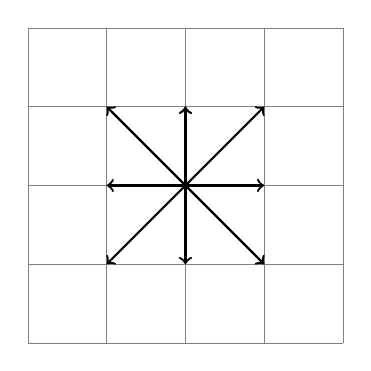
\begin{tikzpicture}
  \draw[step=1cm,gray,very thin] (-2,-2) grid (2,2);
  \draw[thick,->] (0,0) -- (0,1);
  \draw[thick,->] (0,0) -- (1,0);
  \draw[thick,->] (0,0) -- (0,-1);
  \draw[thick,->] (0,0) -- (-1,0);
  \draw[thick,->] (0,0) -- (0,1);
  \draw[thick,->] (0,0) -- (-1,-1);
  \draw[thick,->] (0,0) -- (1,1);
  \draw[thick,->] (0,0) -- (-1,1);
  \draw[thick,->] (0,0) -- (1,-1);
\end{tikzpicture}

\nt{convention: a dot is going towards you(out of the page), a cross is going away from you(into the page).}

\section{Magnetic Force}

\dfn{Magnetic Force}{
  The magnetic force is the force that a magnetic field exerts on a moving charge.
  \\
  The equation for the magnetic force is $ \vec{F} = q \vec{v} \times \vec{B} \sin \alpha  $
  \\
  The direction of the magnetic force is perpendicular to both the velocity and the magnetic field.
}

\thm{Force of a field on a wire}{
  The force of a magnetic field on a wire is $ \vec{F} = BIl  $
  \\
  The direction of the force is perpendicular to both the wire and the magnetic field.
}


\dfn{Cyclotronic Equation}{
  $$ F_c = F_{mag} = \frac{mv^2}{r} = qvB  $$
  $$ \frac{mv^2}{r} = qvB  $$ 
  $$ r = \frac{mv}{qB} $$
}

\qs{Find the magnitude of the magnetic field of a proton \dots}{
 \dots that takes 1.00 $\mu s$ to complete a circlular path. 
  Given that the mass of a proton and the charge of a proton are: 
  $$ m_p = 1.67 \times 10^{-27} kg $$ 
  $$ q_p = 1.6 \times 10^{-19} C $$ 
}

\sol{
}

\thm{Electro-motive force}{
  $$ \epsilon = v l B $$
}

\end{document}
